\documentclass[a4paper]{article}
\usepackage[utf8]{inputenc}
\usepackage{tikz}
\usepackage[top=3cm,left=3cm,right=3cm,bottom=3cm]{geometry}
\usetikzlibrary{shapes.geometric, arrows}

\tikzstyle{startstop} = [rectangle, rounded corners, minimum width=3cm, minimum height=1cm,text centered, draw=black, fill=red!30]
\tikzstyle{io} = [trapezium, trapezium left angle=70, trapezium right angle=110, minimum width=3cm, minimum height=1cm, text centered, draw=black, fill=blue!30]
\tikzstyle{process} = [rectangle, minimum width=3cm, minimum height=1cm, text centered, text width=3cm, draw=black, fill=orange!30]
\tikzstyle{decision} = [diamond, minimum width=3cm, minimum height=1cm, text centered, draw=black, fill=green!30]
\tikzstyle{arrow} = [thick,->,>=stealth]



\title{Programming Fundamentals I - Personal Project}
\author{Report 1 - Pennati Lucas}



\begin{document}
\maketitle
\section{Introduction}
The following document aims to be a small introduction into the logic and planning of the personal project for Programming Fundamentals 1. The topic chosen is ``Display and update information board for the Universit\`a bus stop for the next 30 minutes''.
\section{Planned set of features}
Although the task description does not include any details on what is expected, here follow some of the features that I wish to implement during the duration of the project.
\begin{itemize}
\item Variable departure station\\ In order to achieve this goal, it is important to design the program and the logic behind it in such a way that, if the user wishes, the departure station can be easily modified, and the program adapts to it. This way even if the system is relocated, the adjustments are kept to a minimum.
\item Detailed information\\ The most information possible should be displayed on the screen, without over saturating the space available. The information should include basic key elements such as departure time and line number, as well as some more optional ones such as delays and origin. 
\item Background updates\\
The system should be designed as a zero maintenance tool, reducing what the user has to do to a minimum. This includes designing a way to update the feeds automatically, as well as designing the whole code in a very robust way, capable of handling errors.

\item Graphical User Interface\\
Although the topic description does not ask for one, the project will include a graphical user interface, in order to represent the gathered data in a clear and structured way. The following is a mockup of what could be achieved:\\

\begin{center}
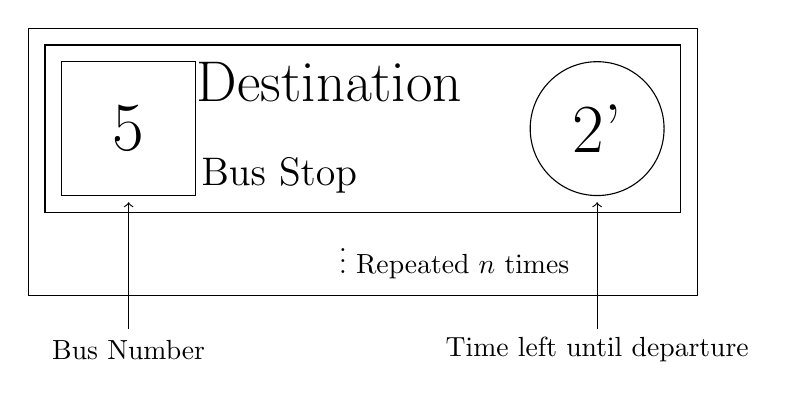
\begin{tikzpicture}[scale=0.85]
\draw (0,2) rectangle (10,6);
%Entry 1
\draw (0.25,3.25) rectangle (9.75,5.75);
\draw (0.5,3.5) rectangle (2.5,5.5);
\draw (8.5,4.5) circle (1);
\draw (8.5,4.5) node {\Huge 2'};
\draw (1.5,4.5) node {\Huge 5};
\draw (4.5,5.2) node {\huge Destination};
\draw (3.75,3.8) node {\Large Bus Stop};

\draw[->] (8.5,1.5) -- (8.5,3.4);
\draw (8.5,1.2) node {Time left until departure};

\draw[->] (1.5,1.5) -- (1.5,3.4);
\draw (1.5,1.2) node {Bus Number};

\draw (4.5,2.6) node[anchor=west] {$\vdots$ Repeated $n$ times};
\end{tikzpicture}
\end{center}
Although quite simplistic, this mockup contains all the information needed at a glance. In order to make it easier to read without spending too much time on it, the time left circle will have three different colors:
\begin{itemize}
\item Green: The circle will be highlighted green when it is sure that the user can catch this bus, including the time taken to get to the bus stop.
\item Yellow: The circle will be highlighted yellow when it is uncertain if the user will be able to catch that connection.
\item Red: The circle will be highlighted red when it is sure that the user will not be able to make it to the bus stop on time. 
\end{itemize}
\item Platform independent\\
Being as there are multiple components, the decisions will also be made based on cross compatibility between platforms, being as this is a great project that could run on a small, low power device such as a Raspberry Pi. In order to achieve this goal, the graphical library Tkinter will be used, and the GUI will be designed to be able to scale adapting to multiple displays.
\end{itemize}

\section{Design Strategy}
In order to implement the planned set of features, the system will have to be designed with robustness in mind, as well as lightness and simplicity. This means that when, for example, fetching data, the program should be able to handle any errors given back by either the APIs, or the HTTP request itself. This idea of robustness is going to be applied to the entire code, in order to be sure that the system will be running even after some major errors and/or problems. Also, the ability to adapt to different screen sizes will be a major point, so to be sure that the code is portable among different platforms and configurations.

\section{Temporary conclusion}
As stated in the introduction, this document aimed at giving a simple overview of the ideas behind such a project, and not a full blown explanation. Although many goals have been set, the challenge is going to be to ensure that everything works, and that it is up to a certain standard, even if this means dropping a feature or two. 

\end{document}






\begin{tikzpicture}[node distance=2cm]

\node (start) [startstop] {Start};
\node (pro1) [process, below of=start] {Process 1};
\node (dec1) [decision, below of=pro1, yshift=-0.5cm] {Decision 1};
\node (pro2a) [process, below of=dec1, yshift=-0.5cm] {Process 2a text text text text text text text text text text};
\node (pro2b) [process, right of=dec1, xshift=2cm] {Process 2b};
\node (out1) [io, below of=pro2a] {Output};
\node (stop) [startstop, below of=out1] {Stop};

\draw [arrow] (start) -- (in1);
\draw [arrow] (in1) -- (pro1);
\draw [arrow] (pro1) -- (dec1);
\draw [arrow] (dec1) -- node[anchor=east] {yes} (pro2a);
\draw [arrow] (dec1) -- node[anchor=south] {no} (pro2b);
\draw [arrow] (pro2b) |- (pro1);
\draw [arrow] (pro2a) -- (out1);
\draw [arrow] (out1) -- (stop);


\end{tikzpicture}
